\section{Systembeskrivelse}


På Ingeniørhøjskolen Aarhus Universitet forefindes en AeroQuad Cyclone ARF quadrocopter. I tidligere projekter er quadrocopteren blevet fjernstyret via line of sight, radiokommunikation. Målet med dette projekt er, at omdanne quadrocopteren til en autonom overvågnings drone.

Groft skitseret består projektet af følgende to dele: 
1. Quadrocopter
2. Webapplikation

Fra projektets start bestod quadrocopteren af et stel, nogle motorer og et batteri. GPS, højdemåler, kamera og 3G modul tilføjes quadrocopteren for at udvide dens funktionalitet. GPS tilføjes, så dronen under flyvning kan tilpasse flyveorientering. For at holde en konstant flyvehøjde tilføjes højdemåler. Kameraet skal bruges til at tage billeder og optage korte filmsekvenser, så det kan dokumenteres hvor dronen har fløjet. Det ønskes, at drone og webapplikation skal kommunikere via internettet, derfor udstyres dronen med et 3G modul.

Webapplikationen har to formål. For det første, skal webapplikation bruges til at indstille nye flyveruter. Nye flyveruter dannes ud fra waypoints som vælges af bruger. Ved indstilling af nye flyveruter skal det også være muligt at indstille flyvehøjde. For det andet skal webapplikationen bruges til at tilgå en database, hvor billeder, film og flyveruter gemmes.

Nederst til højre på systemskitsen ses et device. Dette device har internet adgang og bruges til at tilgå webapplikation hvor opsætning af ny flyvning ordnes.  Når en bruger har lavet indstillinger til ny flyvning, overføres opsætningen via internettet til quadrocopteren. Quadrocopteren finder via GPS ud af hvor den er, og hvor den skal flyve hen. Under flyvningen tager quadrocopteren billeder eller optager video, som via nettet overføres til en database der er tilknyttet webapplikationen.

\vspace{-5pt}
%Systemskitse
\begin{figure}[H]
\centering
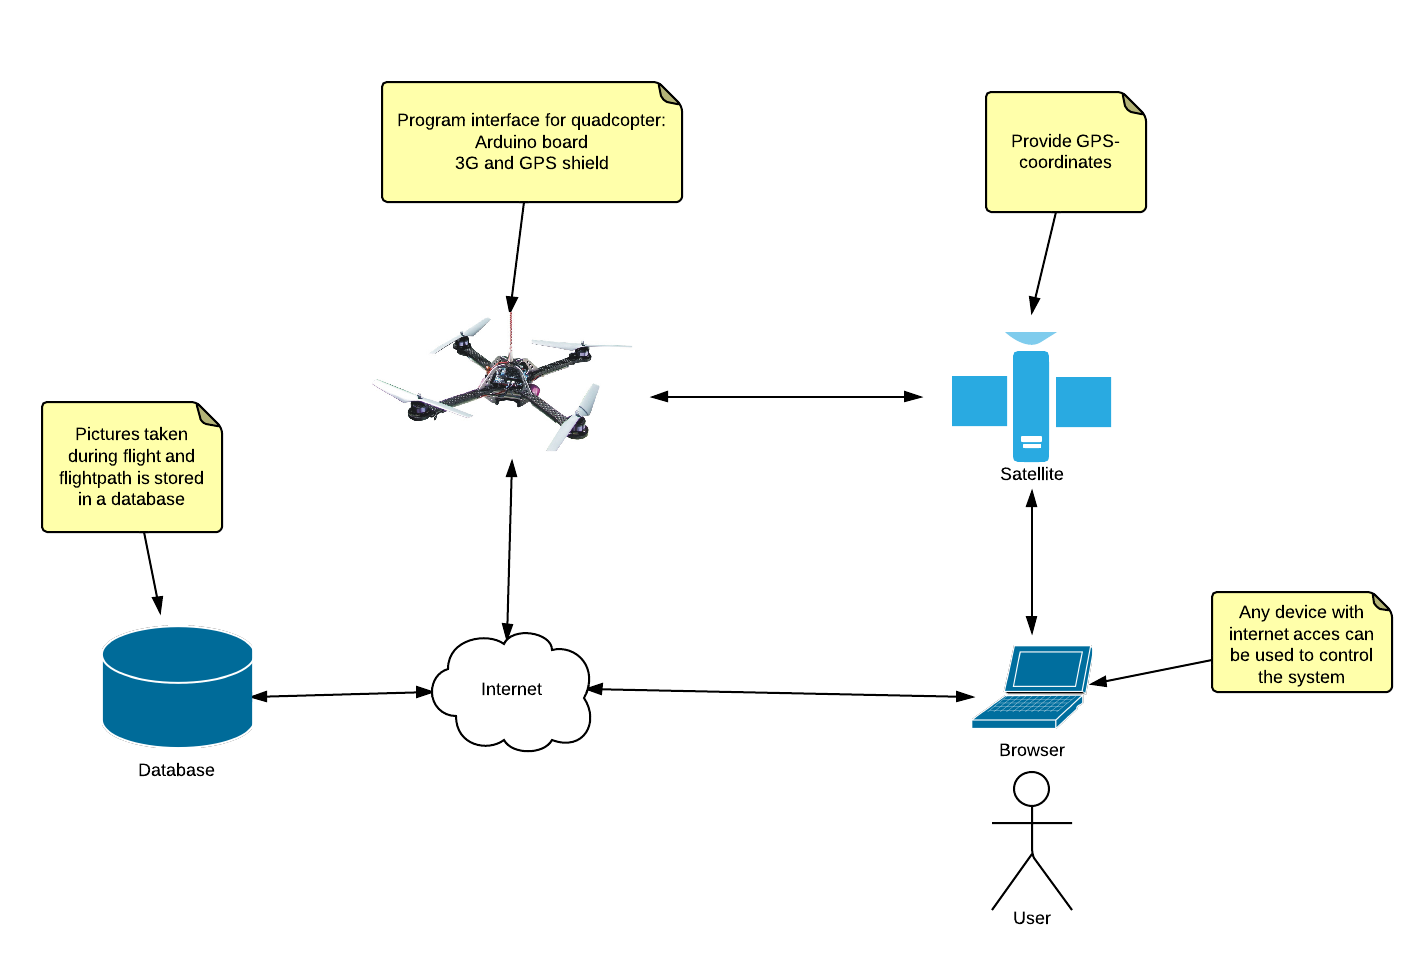
\includegraphics[width=0.7\textwidth]{Billeder/Projektbeskrivelse.png}
\vspace{-5pt}
\caption{Systemskitse}
\label{fig:Systemskitse}
\end{figure}